%%%%%%%%%%%%%%%%%%%%%%%%%%%%%%%%%%%%

\section{1.2.Noções básicas}

%%%%%%%%%%%%%%%%%%%%%%%%%%%%%%%%%%%%

\subsection{Observações e variáveis}

\begin{frame}
\frametitle{Matriz de dados}

\justifying
Abaixo os dados indicam características de estudantes de uma turma de estatística:

\begin{center}
\begin{tabular}{l cccc l}
		& \hl{variável} \\
		& \hl{$\downarrow$}	 \\
\cline{1-5}
No.	&	\var{gênero}	&	\var{intro\_extra} & $\cdots$ & \var{código} \\
\cline{1-5}
1 & masculino & extrovertido  & $\cdots$ & 3 \\ 
  2 & feminino & extrovertido & $\cdots$ & 2 \\ 
  3 & feminino & introvertido  & $\cdots$ & 4 & \hl{$\leftarrow$}  \\ 
  4 & feminino & extrovertido  & $\cdots$ & 2 & \hl{observação} \\
$\vdots$	&	$\vdots$	  &	$\vdots$  &	$\vdots$ &	$\vdots$ \\
86	& masculino & extrovertido & $\cdots$& 3 \\
\cline{1-5}
\end{tabular}
\end{center}

\end{frame}

%%%%%%%%%%%%%%%%%%%%%%%%%%%%%%%%%%%%

\subsection{Tipos de variáveis}

\begin{frame}
\frametitle{Tipos de Variáveis}
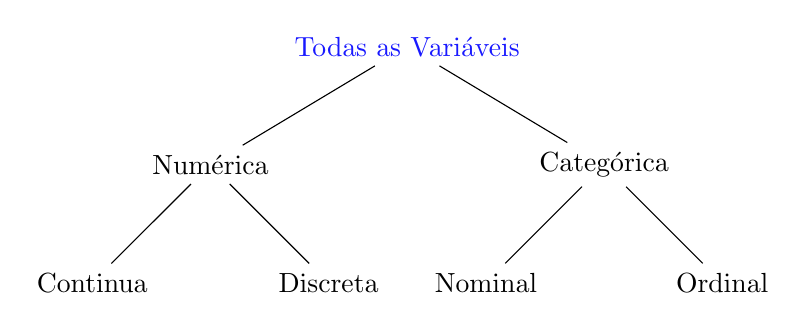
\begin{tikzpicture}
\tikzstyle{level 1} = [sibling distance=5cm]
\tikzstyle{level 2} = [sibling distance=3cm]
\tikzstyle{level 3} = [sibling distance=1cm]

\node{\textcolor{blue!90}{Todas as Variáveis}}
child{
node{Numérica}
        child{
                node{Continua}
                }
        child{
                node{Discreta}
                }        
        }
child{
node{Categórica}
        child{
                node{Nominal}
                }
        child{
                node{Ordinal}
                }        
        };

\end{tikzpicture}

\newline

\end{frame}

%%%%%%%%%%%%%%%%%%%%%%%%%%%%%%%%%%%
\newpage
\begin{frame}
\frametitle{Tipos de Variáveis (cont.)}

\begin{center}
{\footnotesize
\begin{tabular}{c ccc cc}
  \hline
 & \var{gênero} & \var{sono} & \var{hora de dormir} & \var{país} & \var{código} \\
  \hline
1 & masculino & 5 & 12-2 & 13 & 3 \\ 
  2 & feminino & 7 & 10-12 & 7 & 2 \\ 
  3 & feminino & 5.5 & 12-2 & 1 & 4 \\ 
  4 & feminino & 7 & 12-2 &  & 2 \\ 
  5 & feminino & 3 & 12-2 & 1 & 3 \\ 
  6 & feminino & 3 & 12-2 & 9 & 4 \\ 
  \hline
\end{tabular}
}
\end{center}

\begin{itemize}
\item \var{gênero}: \pause \soln{\only<2->{categórica}} \pause
\item \var{sono}: \pause \soln{\only<4->{numérica, contínua}} \pause
\item \var{hora de dormir}: \pause \soln{\only<6->{categórica, ordinal}} \pause
\item \var{país}: \pause \soln{\only<8->{categórica, nominal}} \pause
\item \var{código}: \pause \soln{\only<10->{categórica, ordinal }}
\end{itemize}

\end{frame}

%%%%%%%%%%%%%%%%%%%%%%%%%%%%%%%%%%%

\begin{frame}
\frametitle{Prática}

\pq{Que tipo de variável é um código de área de telefone?}

\begin{enumerate}[(a)]
\item numérico, contínuo
\item numérico, discreto
\solnMult{categórico}
\item categórico, ordinal
\end{enumerate}

\end{frame}

%%%%%%%%%%%%%%%%%%%%%%%%%%%%%%%%%%%

\subsection{Associação entre variáveis}






%%%%%%%%%%%%%%%%%%%%%%%%%%%%%%%%%%%

\begin{frame}
\frametitle{Associação entre variáveis}

\dq{Parece haver alguma relação entre a nota (GPA: 
Grading in education) de um aluno e o número de horas que ele estuda por semana?}

\begin{center}
\cfill 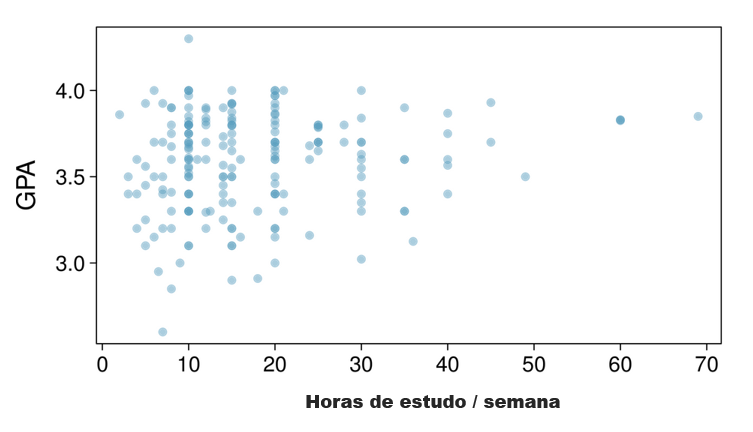
\includegraphics[scale=0.5]{1-2_data_basics/gpa_study_hours.png}
\end{center}

\end{frame}
%%%%%%%%%%%%%%%%%%%%%%%%%%%%%%%%%%%

\begin{frame}
\frametitle{Associação entre variáveis}

\dq{Você consegue identificar algo incomum?}

\soln{\pause{Há um aluno com GPA (nota) $> $ 4,0, isso é provavelmente um erro nos dados.}}

\end{frame}

%%%%%%%%%%%%%%%%%%%%%%%%%%%%%%%%%%%




\subsection{Variáveis dependentes e independentes}

%%%%%%%%%%%%%%%%%%%%%%%%%%%%%%%%%%%

\begin{frame}
\frametitle{Prática}

\twocol{0.5}{0.5}
{
\pq{Com base no gráfico de dispersão, qual das seguintes afirmações sobre comprimentos da cabeça e tamanho do crânio de gambás está correta?}
}
{
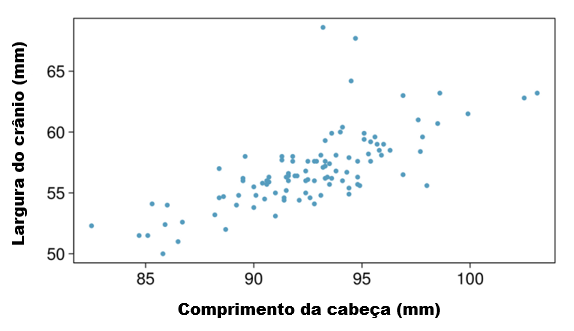
\includegraphics[width=0.7\textwidth]{1-2_data_basics/possum_head_skull.png}
}

\begin{enumerate}[(a)]
\justifying
\item Não existe relação entre o comprimento da cabeça e a largura do crânio, isto é, as variáveis são independentes.
\justifying
\solnMult{O comprimento da cabeça e a largura do crânio estão associadas positivamente.}
\justifying
\item A largura do crânio e o comprimento da cabeça estão associados negativamente.
\justifying
\item Uma cabeça mais longa faz com que o crânio fique mais largo.
\justifying
\item Um crânio mais largo faz com que a cabeça seja mais longa.
\end{enumerate}

\end{frame}

%%%%%%%%%%%%%%%%%%%%%%%%%%%%%%%%%%%

\begin{frame}
\frametitle{Associado vs. independente}

\begin{itemize}
\justifying
\item Quando duas variáveis mostram alguma conexão umas com as outras, elas podem ser chamadas de variáveis \hl{dependentes} e vice-versa.

\justifying
\item Se duas variáveis não estão associadas, ou seja, não há conexão evidente entre as duas, então elas são ditas \hl{independentes}.

\end{itemize}

\end{frame}

%%%%%%%%%%%%%%%%%%%%%%%%%%%%%%%%%%%%
